\documentclass[10pt,twocolumn]{article}

\usepackage[margin=0.72in]{geometry}
\usepackage{amsmath,amssymb,amsfonts,amsthm,mathtools,bm}
\usepackage{graphicx}
\usepackage{booktabs}
\usepackage{enumitem}
\usepackage{xcolor}
\usepackage{float}
\usepackage{hyperref}
\usepackage[nameinlink,capitalise]{cleveref}
\usepackage{microtype}
\usepackage{array}
\usepackage{dblfloatfix}
\usepackage{placeins}

\graphicspath{{figures/}}
\hypersetup{
    colorlinks=true,
    linkcolor=blue!60!black,
    citecolor=blue!60!black,
    urlcolor=blue!60!black,
    pdftitle={Early Gradient Spectra Predict Useful Low-Rank Adaptation},
    pdfauthor={Ruge Lin},
    pdfsubject={Useful-rank prediction and controlled LoRA rank allocation},
    pdfkeywords={LoRA, low-rank adaptation, effective rank, early gradients, rank allocation}
}
\setcounter{dbltopnumber}{3}
\renewcommand{\dbltopfraction}{0.95}
\renewcommand{\textfraction}{0.05}

\newtheorem{theorem}{Theorem}[section]
\newtheorem{proposition}[theorem]{Proposition}
\newtheorem{corollary}[theorem]{Corollary}
\newtheorem{lemma}[theorem]{Lemma}
\theoremstyle{definition}
\newtheorem{definition}[theorem]{Definition}
\newtheorem{remark}[theorem]{Remark}

\newcommand{\R}{\mathbb{R}}
\newcommand{\E}{\mathbb{E}}
\newcommand{\op}{\mathrm{op}}
\newcommand{\F}{\mathrm{F}}
\newcommand{\rank}{\mathrm{rank}}
\newcommand{\argmin}{\mathop{\mathrm{argmin}}}
\newcommand{\half}{\tfrac12}
\newcommand{\DeltaStar}{\Delta_\star}
\newcommand{\Mstar}{M_\star}
\newcommand{\Mhat}{\widehat M}
\newcommand{\eff}{\mathrm{eff}}
\newcommand{\near}{\mathrm{near}}
\newcommand{\rec}{\mathrm{rec}}
\newcommand{\pen}{\mathrm{pen}}
\newcommand{\Id}{I}

\title{Early Gradient Spectra Predict Useful Low-Rank Adaptation}
\author{Ruge Lin}
\date{}

\begin{document}
\maketitle



\begin{abstract}
LoRA and related PEFT methods expose a nominal rank, but useful rank depends on the task spectrum seen through the model's activations.  For a frozen linear map with activation covariance $C$ and task update $\Delta_\star$, we show that the best rank-$r$ adapter is the truncated SVD of $M_\star=\Delta_\star C^{1/2}$ and has excess risk $\frac12\sum_{i>r}\sigma_i^2(M_\star)$.  The activation-whitened population gradient at the frozen model has exactly this spectrum, making early-gradient spectra candidates for predicting useful adapter rank before training.  In five-seed matrix simulations, activation-whitened gradient effective rank predicts a plan-locked near-best useful-rank target with mean in-sample $R^2=0.777$ and mean Spearman correlation $0.852$ in a hard-knee regime; the corresponding sample-limited values are $0.687$ and $0.786$.  We then test the stronger extrapolation from rank prediction to cross-module allocation.  A plan-locked synthetic-transformer study with two task families and ten independent task--seed runs yields a null confirmatory result for soft spectral dimension versus exact-cost uniform allocation: mean loss difference $+0.0146$, 95\% task-stratified bootstrap interval $[-0.0078,0.0352]$, and exact two-sided sign-flip $p=0.2402$.  Separately, a checksum-bound GPT-2/Wikitext-2 study restricted to $c_{attn}$ and $c_{fc}$ modules finds a small but consistent improvement over exact-cost uniform rank 4 in all eight plan-locked primary seeds: mean paired loss difference $-0.0070$, bootstrap interval $[-0.0083,-0.0060]$, exact $p=0.0078$, and within-suite Holm-adjusted $p=0.0391$.  Adding attention output projections reverses direction in a three-seed boundary suite ($+0.0011$, 0/3 wins).  Thus early-gradient spectra predict useful rank and can support allocation in a controlled module scope, but the synthetic null, rank--scale sensitivity, and boundary reversal rule out a universal allocator claim.
\end{abstract}

\paragraph{Scope and claim boundary.}
Most evidence is theorem-driven and synthetic.  The central empirical claim is useful-rank prediction in matrix simulations, not universal rank allocation in transformers.  The corrected synthetic-transformer experiment yields a null confirmatory result under its primary fixed-scale condition.  The real-model primary result is confirmatory only for one frozen GPT-2 checkpoint, one dataset, one short-training protocol, and the plan-locked $c_{attn}/c_{fc}$ module suite; its attention-output-projection boundary suite reverses direction.  We do not claim nonlinear transformer convergence, broad model or task generalization, or unconditional dominance of a spectral allocator.

% -----------------------------------------------------------------------------
\section{Introduction}
\label{sec:intro}

Low-rank adaptation methods such as LoRA make rank a visible and tunable resource.  A rank-$r$ LoRA adapter learns
\begin{equation}
    \Delta W = \frac{\alpha}{r}BA,
\end{equation}
with $B\in\mathbb R^{d_{\rm out}\times r}$ and $A\in\mathbb R^{r\times d_{\rm in}}$.  In practice, however, nominal rank is an incomplete description of adaptation capacity.  Rank interacts with scale, optimization time, activation geometry, finite-sample noise, and the module on which the adapter is placed.  A rank that is algebraically available may not be functionally useful, and a small budget spent on the right module can outperform a larger budget spread uniformly.

We separate \emph{nominal rank} from \emph{useful rank}.  Nominal rank is the algebraic rank supplied to the adapter.  Useful rank is the smallest rank satisfying a practical criterion: near-best validation loss, a fixed fraction of attainable improvement, or a rank-penalized tradeoff.  Our central observation is that useful rank is a spectral quantity in function space.  If $C$ is the activation covariance and $\Delta_\star$ is the task update, the relevant operator is
\begin{equation}
    M_\star = \Delta_\star C^{1/2}.
\end{equation}
This activation weighting discounts update directions that the model rarely uses.

We prove two exact population statements in a reduced-rank adaptation model.  First, the best rank-$r$ adapter is obtained by truncating the singular spectrum of $M_\star$.  Second, the early full gradient at the frozen model, after activation whitening, equals $-M_\star$.  Therefore, the useful-rank spectrum is visible before training an adapter.  We validate this prediction in controlled matrix simulations.  We then test a stronger, non-equivalent hypothesis: whether a scalar spectral score can allocate a fixed LoRA parameter budget across transformer modules.  A plan-locked ten-run study with exact-cost comparators and common random numbers does not show a confirmatory advantage for the primary spectral allocator, and sitewise score--rank relationships reverse sign across the two task families.  This negative bridge result is informative because it separates theorem-supported rank prediction from a practical allocation heuristic that requires further structure.

\paragraph{Contributions.}
\begin{enumerate}[leftmargin=1.4em,itemsep=1pt]
    \item We give an exact reduced-rank adaptation theorem: rank-$r$ excess risk is the tail singular energy of $\Delta_\star C^{1/2}$.
    \item We show that the activation-whitened population early gradient has the same spectrum as this task operator.
    \item We define useful-rank targets--near-best, recovery, and penalized rank--that avoid the degeneracy of unconstrained best rank.
    \item We validate useful-rank prediction in multi-seed spiked matrix simulations, where gradient effective rank strongly predicts practical rank targets.
    \item We conduct a plan-locked synthetic-transformer allocation study with ten independent task--seed runs, exact-cost baselines, common random numbers, three adaptation replicates, and explicit scaling controls; its null confirmatory result identifies a boundary between rank prediction and module allocation.
    \item We conduct a checksum-bound GPT-2/Wikitext-2 study with eight plan-locked primary seeds, exact-cost and common-random-number controls, allocation-only adaptive baselines, and a separate three-seed module-family boundary suite; the primary gain is statistically resolved but practically small, and the boundary suite reverses direction.
\end{enumerate}

% -----------------------------------------------------------------------------
\section{Related Work}
\label{sec:related}

\paragraph{LoRA and PEFT.}
LoRA freezes pretrained weights and trains low-rank increments, giving strong fine-tuning performance with far fewer trainable parameters \cite{hu2021lora}.  QLoRA backpropagates through quantized frozen models into LoRA adapters, making LoRA-style adaptation central to memory-efficient fine-tuning \cite{dettmers2023qlora}.  Our focus is orthogonal: how much low-rank capacity is useful, and how should it be allocated?

\paragraph{Adaptive rank and scaling.}
AdaLoRA explicitly reallocates rank budget across weight matrices using importance scores \cite{zhang2023adalora}.  DyLoRA trains LoRA blocks over a range of ranks so that one checkpoint can expose multiple usable ranks without a separate exhaustive rank search \cite{valipour2023dylora}.  Rank-stabilized LoRA changes the standard $\alpha/r$ scaling to mitigate high-rank learning issues \cite{kalajdzievski2023rslora}.  DoRA decomposes weights into magnitude and direction and applies low-rank updates to the direction component \cite{liu2024dora}.  These works motivate rank allocation and rank-scale disentanglement.  We contribute a pre-training spectral predictor of rank demand rather than a dynamic-rank adapter training method.

\paragraph{Data- and gradient-driven rank allocation.}
EVA uses activation singular vectors for LoRA initialization and redistributes rank according to explained activation variance \cite{paischer2025eva}.  GoRA combines gradient-driven rank adaptation with adaptive initialization \cite{he2025gora}, while FIM-LoRA allocates rank from calibration-time gradient variance on LoRA-$B$ parameters \cite{sathyavageeswaran2026fimlora}.  ShapLoRA estimates rank importance with a Shapley-value-inspired sensitivity score on a validation set and an allocation--retraining workflow \cite{zhao2026shaplora}.  Our GPT-2 comparisons isolate allocation rather than reproduce these full methods: the EVA-, GoRA-, and FIM-LoRA-style controls use their corresponding score families but share the same nested initialization, exact parameter cost, stochastic streams, optimizer, and training schedule as every other strategy.

\paragraph{Gradient subspaces and spectral perturbation.}
LoRA-One studies one-step full-gradient subspaces and shows that singular directions of the gradient can guide low-rank adaptation \cite{zhang2025loraone}.  We ask a complementary question: not only which subspace, but how many directions.  Xu et al. analyze LoRA learning dynamics for matrix factorization under gradient flow, emphasizing initialization-dependent convergence and spectral initialization guarantees \cite{xu2025loradynamics}.  Our reduced-rank result is complementary: it identifies the useful-rank spectrum through the activation-whitened population gradient.  Mathematically, we build on Eckart--Young--Mirsky low-rank approximation \cite{eckart1936approximation,mirsky1960symmetric}, classical perturbation theory \cite{davis1970rotation}, and spiked random-matrix transitions \cite{benaych2012singular}.  Pythia is a natural future open-model validation suite because it provides controlled checkpoints across scale and training time \cite{biderman2023pythia}; we do not use it in this paper.

% -----------------------------------------------------------------------------
\section{Theory}
\label{sec:theory}

Let
\begin{align}
    y&=(W_0+\DeltaStar)x+\xi,\\
    \E[x]&=0,\qquad \E[xx^\top]=C\succ0,\qquad \E[\xi\mid x]=0.
\end{align}
A rank-constrained adapter predicts $(W_0+\Delta)x$ with $\rank(\Delta)\le r$, and
\begin{equation}
    \mathcal L(\Delta)=\half\E\|y-(W_0+\Delta)x\|_2^2.
\end{equation}
Define $\Mstar=\DeltaStar C^{1/2}$.

\begin{theorem}[Population reduced-rank adaptation]
\label{thm:population}
Let $\Mstar=U\Sigma V^\top$ with singular values $\sigma_1\ge\sigma_2\ge\cdots$.  The best rank-$r$ adapter is
\begin{equation}
    \Delta_r^\star=U_r\Sigma_rV_r^\top C^{-1/2},
\end{equation}
and its excess risk is
\begin{equation}
    \mathcal L(\Delta_r^\star)-\mathcal L(\DeltaStar)=\half\sum_{i>r}\sigma_i^2(\Mstar).
\end{equation}
\end{theorem}

The smallest rank recovering fraction $\rho$ of the attainable improvement is
\begin{equation}
    r_{\rec}(\rho)=\min\left\{r:\sum_{i\le r}\sigma_i^2(\Mstar)\ge \rho\sum_i\sigma_i^2(\Mstar)\right\}.
\end{equation}

\begin{proposition}[Early-gradient spectrum]
\label{prop:early-gradient}
Let $G_0=\nabla_\Delta\mathcal L(0)$.  Then
\begin{equation}
    G_0=-\DeltaStar C,\qquad -G_0C^{-1/2}=\DeltaStar C^{1/2}=\Mstar.
\end{equation}
Thus the activation-whitened early gradient has the spectrum that determines useful rank.
\end{proposition}

\paragraph{Predictors.}
We compare hard detectable rank, stable rank, effective rank, and soft spectral dimensions.  The strongest replicated predictor is effective rank:
\begin{equation}
    r_{\eff}(A)=\exp\left(-\sum_i p_i(A)\log p_i(A)\right),\quad p_i(A)=\frac{\sigma_i^2(A)}{\|A\|_F^2}.
\end{equation}
A threshold-aware continuous alternative is
\begin{equation}
    d_{\phi,\tau}(A)=\sum_i\phi\left(\frac{\sigma_i^2(A)}{\tau^2}\right).
\end{equation}
Hard detectable rank corresponds to the discontinuous gate $\phi(t)=\mathbf 1\{t>1\}$.

\paragraph{Finite samples.}
With empirical gradient $\widehat G_0$, ideal whitening gives $\Mhat=-\widehat G_0C^{-1/2}=\Mstar+E$.  If $\|E\|_{\op}\le\varepsilon$, Weyl's inequality controls singular values.  Hard thresholding is stable only with a gap around the edge; effective rank is continuous under relative Frobenius perturbation.  In practice we use regularized empirical whitening:
\begin{equation}
    \widehat M_\lambda=-\widehat G_0(\widehat C+\lambda I)^{-1/2}.
\end{equation}

% -----------------------------------------------------------------------------
\section{Experimental Setup}
\label{sec:setup}

The matrix and small-transformer experiments are synthetic and require no external datasets.  The final GPT-2/Wikitext-2 study uses checksum-pinned local model and dataset files and executes offline to test whether the diagnostic survives one real pretrained-transformer setting.  The goal is to separate useful-rank prediction from cross-module allocation under controlled task spectra, sample noise, rank grids, scale choices, stochastic streams, and exact parameter costs.  Table~\ref{tab:settings} summarizes the experimental regimes.

\begin{table*}[t]
\centering
\small
\caption{Experimental settings.  Stage4 is the primary evidence for early-gradient useful-rank prediction.}
\label{tab:settings}
\begin{tabular}{p{0.16\linewidth}p{0.22\linewidth}p{0.25\linewidth}p{0.27\linewidth}}
\toprule
Experiment & Regime & Sweep & Purpose \\
\midrule
BBP & $m=n=128$, rank-1 spike & spike strength $\theta$ & verify spectral detectability transition \\
LoRA rank & $d_{in}=d_{out}=128$, task rank 8 & ranks $1$--$64$ & test nominal rank and final adapter spectra \\
Alpha / rank-alpha & noisy or rank-8 tasks & $\alpha$ and rank grids & separate rank, scale, and instability \\
Merge/conflict & paired task vectors & overlap/sign sweeps & test signed versus unsigned interference \\
Layerwise hard-knee & 48 synthetic layers & ranks $1$--$32$ & test early-gradient useful-rank prediction \\
Layerwise sample-limited & fewer samples and more noise & ranks $1$--$32$ & test finite-sample degradation \\
Stage4 replication & 5 seeds $\times$ 2 regimes & 48 layers per seed & multi-seed validation \\
Synthetic transformer & 2 tasks $\times$ 5 seeds; 3 adaptation replicates & ranks $0$--$16$, 3 scale rules, exact-cost budgets & test whether spectral rank demand transfers to module allocation \\
GPT-2/Wikitext-2 & 8 primary + 3 boundary seeds & six exact-cost strategies, fixed scale, controlled RNG streams & confirmatory restricted-scope transfer and module-family boundary test \\
\bottomrule
\end{tabular}
\end{table*}

\paragraph{Synthetic regression.}
Tasks use $y=(W_0+\DeltaStar)x+\xi$.  Default dimensions are $d_{in}=d_{out}=128$ with power-law activation covariance.  The main task-rank-8 spike values are
\begin{equation}
    (2.8,2.2,1.8,1.45,1.1,0.85,0.65,0.5).
\end{equation}
LoRA factors are trained by gradient descent with clipping.  Detection thresholds use a permutation null at quantile $0.995$.

\paragraph{Useful-rank targets.}
Let $\mathcal R$ be the tested nominal-rank grid.  For validation curve $V(r)$, define $V_0=V(0)$, $V_{\min}=\min_{r\in\mathcal R}V(r)$, $\Delta V=V_0-V_{\min}$, and $Q(r)=(V_0-V(r))/\Delta V$.  When $\Delta V>0$, we report
\begin{align}
    r_{\near}(\gamma)&=\min\{r\in\mathcal R:V(r)\le V_{\min}+\gamma\Delta V\},\nonumber\\
    r_{\rec}(\rho)&=\min\{r\in\mathcal R:Q(r)\ge\rho\},\nonumber\\
    r_{\pen}(\lambda)&=\argmin_{r\in\mathcal R}\{V(r)+\lambda\Delta V r/r_{\max}\}.\nonumber
\end{align}
Ties are resolved in favor of the smallest nominal rank.  Curves with $\Delta V\le0$ have undefined useful-rank targets and are excluded from target fits.  The simulation oracle loss is retained only as a diagnostic and never enters $V_{\min}$, $\Delta V$, a threshold, or a penalty.  The unconstrained observed-best rank is likewise diagnostic; in layerwise experiments it is often the largest rank tested.

% -----------------------------------------------------------------------------
\section{Results}
\label{sec:results}

\subsection{Detectability and nominal-rank failures}

The BBP-style simulation confirms the expected detectability transition (Figure~\ref{fig:early-results}, left).  In rank-1 Gaussian noise with edge near $2.0$, planted/empirical overlap is near zero for small spikes and rises after spectral separation: mean overlap is about $0.008$ at $\theta=0.1$, $0.288$ at $\theta=1.2$, $0.540$ at $\theta=1.5$, and $0.893$ at $\theta=3.0$.

\begin{figure*}[t]
\centering
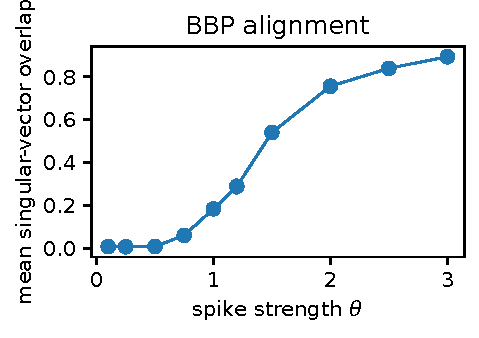
\includegraphics[width=0.32\linewidth]{bbp_alignment_summary.pdf}
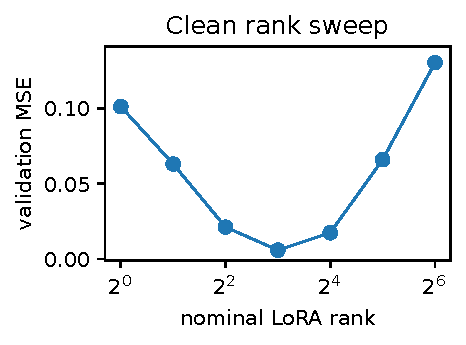
\includegraphics[width=0.32\linewidth]{lora_rank_clean_val_loss.pdf}
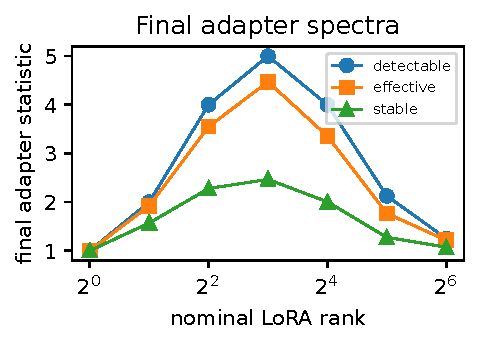
\includegraphics[width=0.32\linewidth]{lora_rank_clean_spectral_stats.pdf}
\caption{Left: BBP detectability transition.  Middle: a clean fixed-$\alpha$ LoRA rank sweep is U-shaped, so nominal rank is not the explanatory variable.  Right: final adapter spectral statistics peak near the useful-rank range.}
\label{fig:early-results}
\end{figure*}

The rank-sweep panels in Figure~\ref{fig:early-results} show why nominal rank alone is insufficient.  A cleaned fixed-$\alpha$ LoRA sweep with $\alpha=16$, learning rate $0.2$, 1200 steps, ranks $1$--$64$, and 8 repetitions shows a U-shaped curve.  Mean validation loss is $0.1011$ at rank 1, $0.0211$ at rank 4, $0.0058$ at rank 8, $0.0174$ at rank 16, and $0.1303$ at rank 64.  Robust fits show that final adapter stable/effective/detectable rank explain validation loss far better than nominal rank.

\subsection{Rank and scale are confounded}

Alpha controls both optimization and drift.  In the alpha stress run, validation loss improves up to moderate $\alpha$ and then degrades mildly, while the output-drift proxy increases.  Large $\alpha$ did not robustly create separate ``intruder'' directions in this synthetic setting; the safer interpretation is amplification and drift.  A rank-alpha grid further shows that nominal rank alone is weak: on the clean subset with validation loss $<1$, adapter stable rank reaches $R^2\approx0.810$ for log validation loss, adapter detectable rank plus alpha reaches $R^2\approx0.778$, adapter effective rank reaches $R^2\approx0.740$, alpha alone reaches $R^2\approx0.552$, and nominal rank alone reaches only $R^2\approx0.040$.

\subsection{Signed conflict is secondary but informative}

The original unsigned merge-overlap experiment was weak: spectral interference explained only about $R^2=0.051$ for merge degradation and planted overlap about $R^2=0.046$.  A corrected signed-conflict experiment gave a clearer story: the signed task inner product explains merge degradation with $R^2=0.9995$, while a conflict score gives $R^2=0.747$ and unsigned overlap alone gives $R^2=0.085$.  This is a secondary result; it supports using signed spectral geometry rather than unsigned overlap for task-vector interference.

\subsection{Stage4: early-gradient effective rank predicts useful rank}

The main matrix-simulation evidence is the Stage4 replication: five seeds per condition and 48 synthetic layers per seed.  For each layer, we compute activation-whitened early-gradient spectral statistics, run rank sweeps over $\{1,2,4,8,16,32\}$, and evaluate useful-rank targets.  After pilot-informed protocol development and before the corrected rerun, we froze the hard-knee $r_{\near}(0.1)$ versus activation-whitened gradient effective-rank comparison as the primary confirmatory pair; its sample-limited counterpart is a plan-locked robustness check.  Other displayed targets and all alternative predictors are secondary or exploratory.  Figure~\ref{fig:stage4} and Table~\ref{tab:stage4} report the replicated activation-whitened effective-rank predictor.  The reported Stage4 $R^2$ values are in-sample fits over layer-level targets; corresponding leave-one-out values for the primary hard-knee and sample-limited rows are $0.7547$ and $0.6617$, respectively.

\begin{figure}[t]
\centering
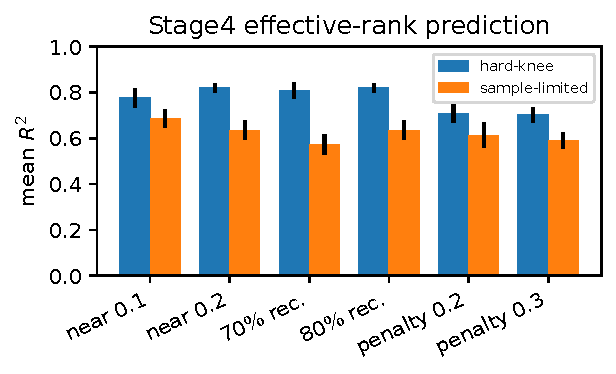
\includegraphics[width=0.95\linewidth]{stage4_effective_rank_r2.pdf}
\caption{Stage4 replication.  Bars show mean in-sample $R^2$ over 5 seeds for activation-whitened gradient effective rank predicting log2 useful-rank targets.  Hard-knee spectra are strongly predicted; sample-limited spectra are weaker but still informative.}
\label{fig:stage4}
\end{figure}

\begin{table}[H]
\centering
\scriptsize
\setlength{\tabcolsep}{2.4pt}
\caption{Stage4 activation-whitened effective-rank results.  Mean over five seeds; SEM in parentheses.}
\label{tab:stage4}
\begin{tabular}{@{}llcc@{}}
\toprule
Condition & Target & Mean in-sample $R^2$ & Mean $\rho$ \\
\midrule
Hard-knee & near-best 0.1 gap & 0.792 (0.038) & 0.848 (0.017) \\
Hard-knee & near-best 0.2 gap & 0.811 (0.021) & 0.853 (0.011) \\
Hard-knee & 70\% recovery & 0.762 (0.031) & 0.856 (0.017) \\
Hard-knee & 80\% recovery & 0.734 (0.043) & 0.841 (0.026) \\
Hard-knee & penalty 0.2 & 0.712 (0.038) & 0.797 (0.029) \\
Hard-knee & penalty 0.3 & 0.714 (0.037) & 0.808 (0.023) \\
\midrule
Sample-limited & near-best 0.1 gap & 0.685 (0.028) & 0.786 (0.022) \\
Sample-limited & near-best 0.2 gap & 0.548 (0.070) & 0.698 (0.057) \\
Sample-limited & 70\% recovery & 0.622 (0.034) & 0.784 (0.026) \\
Sample-limited & 80\% recovery & 0.584 (0.053) & 0.718 (0.041) \\
Sample-limited & penalty 0.2 & 0.554 (0.060) & 0.674 (0.049) \\
Sample-limited & penalty 0.3 & 0.574 (0.037) & 0.703 (0.019)
\\
\bottomrule
\end{tabular}
\end{table}

The hard-knee regime uses $n_{train}=1024$, label noise $0.05$, and weak-factor range $0.01$--$0.08$.  The sample-limited regime uses $n_{train}=384$, label noise $0.12$, and weak-factor range $0.05$--$0.25$.  The unconstrained best rank is degenerate: rank 32 is best for almost every layer.  Useful-rank targets are nondegenerate and predictable.

\FloatBarrier

% -----------------------------------------------------------------------------
\section{Synthetic-Transformer Allocation Test}
\label{sec:transformer-results}

We next test a stronger claim than the matrix theorem: whether modulewise early-gradient spectra can allocate a limited LoRA budget inside a nonlinear transformer.  The study was frozen before the full run and is conditional on two named synthetic task families.  Each independent unit is one task/base-model seed run; budgets and adaptation replicates are nested observations rather than additional independent samples.

\paragraph{Model, tasks, and calibration.}
Each run trains a two-layer decoder-only transformer with $d_{\rm model}=64$, four attention heads, MLP width 128, and zero dropout on a base task, freezes it, and adapts to a shifted task.  Modular arithmetic changes an offset under modulus 31 and exposes eight $q$, $v$, $o$, and MLP-output sites.  Associative recall changes a 16-key mapping and exposes ten sites, additionally including $k$ projections.  For site $j$, hooks estimate
\begin{equation}
    \widehat C_j=\frac1{N_j}\sum_{b,a}x_{j,b,a}x_{j,b,a}^{\top},\qquad
    \widehat G_j=\frac1{B_j}\sum_b\sum_a \widetilde g_{j,b,a}x_{j,b,a}^{\top},
\end{equation}
and form $\widehat M_{j,\lambda}=-\widehat G_j(\widehat C_j+\lambda_j I)^{-1/2}$ with diagonal whitening and $\lambda_j=0.01\operatorname{tr}(\widehat C_j)/d_j$.  Calibration uses eight batches of size 128, 4,096 permutation-null maxima per site, a 0.995 edge quantile, and 2,000 edge-uncertainty resamples.  Rank sweeps use $\{0,1,2,4,8,16\}$.

\paragraph{Plan-locked comparison and controls.}
The primary allocation rule is soft spectral dimension under fixed update scale, compared with a deterministic uniform allocation constructed at the same realized trainable-parameter cost for every candidate allocation.  Standard $\alpha/r$ and rsLoRA are separate sensitivity conditions.  Adapter initialization, training batches, evaluation examples, and all declared random streams are shared across paired rules.  Modular arithmetic is evaluated exhaustively.  Each budget has three adaptation replicates; the six modular and seven associative-recall budgets are first averaged within a task--seed run.  Five independent seeds per task are then averaged within task, and the confirmatory omnibus estimate weights the two task means equally.  Inference uses 10,000 within-task run bootstrap resamples and an exact two-sided task-stratified sign-flip test over all $2^{10}$ patterns; the exact test conditions on the observed magnitudes and assumes sign exchangeability of paired run effects under the null.

\begin{figure*}[t]
\centering
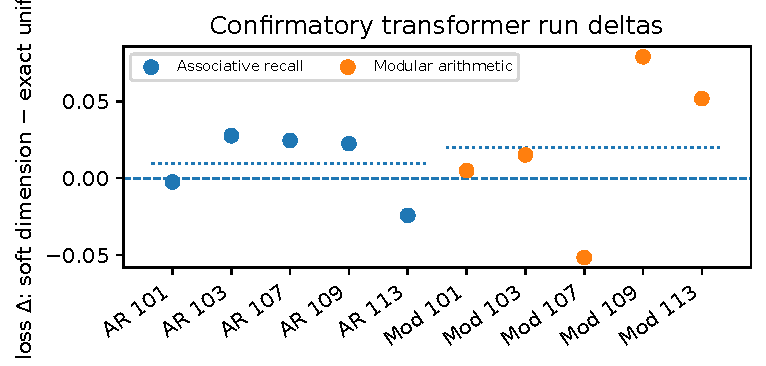
\includegraphics[width=0.78\linewidth]{transformer_primary_run_deltas.pdf}
\caption{Confirmatory synthetic-transformer run effects.  Each point is one independent task--seed run after averaging three adaptation replicates and the plan-locked budgets.  The outcome is final-validation-loss $\Delta=$ soft dimension minus its exact-cost uniform comparator, so positive values favor uniform allocation.  Dotted segments are task means; the dashed line is zero.}
\label{fig:transformer-primary}
\end{figure*}

\begin{table*}[t]
\centering
\small
\caption{Plan-locked fixed-update-scale transformer comparison.  Positive loss $\Delta$ means the soft-dimension candidate is worse than exact-cost uniform allocation.  The omnibus interval resamples independent runs within task and weights task means equally; $p$ values are exact two-sided sign-flip tests under sign exchangeability.  Task-specific rows are secondary and have five-run resolution.}
\label{tab:transformer-primary}
\begin{tabular}{lrrrrrr}
\toprule
Analysis & Runs & Mean loss $\Delta$ & 95\% CI & Exact $p$ & Runs better & Mean acc. $\Delta$ \\
\midrule
\input{tables/generated/transformer_primary_rows.tex}\\
\bottomrule
\end{tabular}
\end{table*}

\paragraph{Confirmatory result.}
Figure~\ref{fig:transformer-primary} and Table~\ref{tab:transformer-primary} do not support an allocation advantage.  The equal-task-weighted loss difference is $+0.0146$ (95\% CI $[-0.0078,0.0352]$, exact $p=0.2402$), with 3/10 run wins and 0/2 task-family mean wins.  The mean accuracy difference is $-0.0039$.  Associative recall has mean loss $\Delta=+0.0095$ and modular arithmetic $+0.0198$; both intervals include zero.  The release contains 2,925 exact-cost candidate pairs, no realized-cost mismatch, no paired-seed disagreement, no divergent row, and zero metric spread among identical allocations, so the null result is not explained by the randomization and cost defects that invalidated the earlier analysis.

\begin{table*}[t]
\centering
\small
\caption{Scaling sensitivity for soft dimension versus exact-cost uniform allocation.  Fixed update scale is confirmatory; standard $\alpha/r$ and rsLoRA are exploratory.  Negative loss $\Delta$ favors the spectral candidate.  None of the exact two-sided tests reaches 0.05.}
\label{tab:transformer-scaling}
\begin{tabular}{llrrrrr}
\toprule
Scaling & Role & Omnibus loss $\Delta$ & Exact $p$ & Runs better & Assoc. $\Delta$ & Modular $\Delta$ \\
\midrule
Fixed update scale & Primary & $+0.0146$ & $0.2402$ & $3/10$ & $+0.0095$ & $+0.0198$ \\
Standard $\alpha/r$ & Exploratory & $-0.0340$ & $0.1973$ & $6/10$ & $-0.0293$ & $-0.0388$ \\
rsLoRA & Exploratory & $+0.0113$ & $0.4609$ & $3/10$ & $-0.0004$ & $+0.0231$
\\
\bottomrule
\end{tabular}
\end{table*}

\paragraph{Scaling and task heterogeneity.}
Table~\ref{tab:transformer-scaling} shows that the direction changes with the LoRA scaling rule.  Under standard $\alpha/r$, the exploratory mean is $-0.0340$ with 6/10 run wins and both task means negative, but the exact $p$ value is $0.1973$; rsLoRA is near zero overall.  This is evidence of rank--scale sensitivity, not evidence for selecting the most favorable condition after observing outcomes.

\begin{table}[H]
\centering
\small
\caption{Sitewise association between spectral score and the near-best 0.1-gap useful-rank target under fixed update scale.  Values are mean Spearman correlations over five independent runs, with SEM.}
\label{tab:transformer-sitewise}
\begin{tabular}{llrr}
\toprule
Task & Predictor & Mean $\rho$ & SEM \\
\midrule
\input{tables/generated/transformer_sitewise_rows.tex}\\
\bottomrule
\end{tabular}
\end{table}

Table~\ref{tab:transformer-sitewise} further separates module importance from rank demand.  Effective rank and soft dimension correlate positively with useful rank in modular arithmetic but negatively in associative recall.  A module can have a strong early-gradient spectrum yet achieve most of its attainable gain at low rank; a scalar score need not simultaneously encode whether a site matters and how many directions it needs.

\paragraph{Superseded analyses.}
The former six-cluster, 39-budget ``33/39 wins'' summary and its one-seed-per-task whitening ablation were generated before common-random-number and exact-cost controls.  They are not publication evidence, are not inputs to any current table or figure, and are omitted from the claims.  Whitening remains theoretically motivated, but its transformer allocation effect must be rerun under the corrected protocol.

\FloatBarrier


% -----------------------------------------------------------------------------
\section{Real GPT-2/Wikitext Validation}
\label{sec:real-gpt2}

The real-model study uses a checksum-pinned local GPT-2 checkpoint and local Wikitext-2 files \cite{radford2019language,merity2016pointer}.  Each source run is executed offline and trains for 200 steps with block size 128, batch size 4, eight calibration batches, and 32 evaluation batches.  Calibration is dropout-free while retaining gradients.  Model, adapter, data, dropout, and evaluation random streams are named and separated; the training RNG is reset after allocation-dependent adapter construction.  All strategies use module-name-derived nested initialization, fixed update scale, and exactly matched trainable-parameter cost.  A duplicate-uniform identity control must match the uniform run in assignment, trace, final adapter state, and evaluation metrics, and every strategy must pass nonzero gradient and adapter-update gates.

The six paper-facing strategies are exact-cost uniform rank 4, activation-whitened spectral effective rank, gradient norm, and allocation-only EVA-, GoRA-, and FIM-LoRA-style controls.  The last three borrow only a scoring family from the corresponding method; they are not full reproductions of those methods' initialization or training algorithms.  The plan-locked primary suite adapts GPT-2 \texttt{c\_attn} and \texttt{c\_fc} modules over eight independent base seeds.  A separate three-seed boundary suite adds \texttt{attn.c\_proj}; it is not pooled with the primary analysis.

\begin{table*}[t]
\centering
\scriptsize
\caption{Controlled GPT-2/Wikitext-2 allocation study.  Final validation loss is mean over independent seeds with SEM in parentheses.  Loss differences are candidate minus exact-cost uniform rank 4, so negative is better.  Intervals are deterministic run-level bootstrap 95\% intervals; wins count lower-loss runs versus uniform.  Every strategy has exactly 331,776 trainable parameters in the primary suite and 405,504 in the boundary suite.}
\label{tab:real-gpt2}
\begin{tabular}{llrrrr}
\toprule
Setting & Strategy & Final val. loss & Loss $\Delta$ vs. uniform & Bootstrap 95\% CI & Wins \\
\midrule
$c_{attn},c_{fc}$ & spectral effective & 3.4573 (0.0016) & 31.73 & 331776 & 4/5 \\
$c_{attn},c_{fc}$ & uniform rank 4 & 3.4587 (0.0017) & 31.78 & 331776 & 1/5 \\
$c_{attn},c_{fc}$ & gradient norm & 3.5047 (0.0014) & 33.27 & 330086 & 0/5 \\
$+a_{proj}$ & spectral effective & 3.4530 (0.0026) & 31.60 & 404992 & 0/3 \\
$+a_{proj}$ & uniform rank 4 & 3.4479 (0.0006) & 31.44 & 405504 & 3/3 \\
$+a_{proj}$ & gradient norm & 3.4847 (0.0014) & 32.61 & 405248 & 0/3 \\
\\
\bottomrule
\end{tabular}
\end{table*}

In the plan-locked $c_{attn},c_{fc}$ primary suite, spectral-effective allocation has mean final validation loss $3.4513$ (SEM $0.0010$), versus $3.4583$ ($0.0012$) for exact-cost uniform rank 4.  The paired mean difference is $-0.007026$ with bootstrap 95\% interval $[-0.008343,-0.006026]$, and spectral allocation wins all eight seeds.  The exact two-sided sign-flip test gives $p=0.0078125$; with eight nonzero paired differences this is the minimum attainable two-sided value under the sign-exchangeability null.  Adjustment across the five plan-locked within-suite candidate comparisons gives Holm $p=0.0390625$.  The absolute effect is small: the loss change corresponds to about $0.70\%$ lower perplexity and about $1.43\%$ of the improvement of exact-cost uniform rank 4 over the frozen model.  EVA-style allocation is also better than uniform in all eight seeds ($-0.004610$, interval $[-0.004911,-0.004315]$), but spectral allocation has the lower mean loss.  GoRA-style, gradient-norm, and FIM-LoRA-style allocations are worse than uniform by $+0.002683$, $+0.027467$, and $+0.041326$, respectively, under this common protocol.

The boundary suite reverses the primary direction.  After adding \texttt{attn.c\_proj}, spectral-effective allocation is worse than uniform in all three seeds: mean difference $+0.001087$ with bootstrap interval $[0.000873,0.001330]$.  The exact two-sided sign-flip value is $p=0.25$, the minimum attainable with three nonzero paired differences, so this suite is descriptive rather than a separately powered confirmatory test.  All other nonuniform controls also lose all three boundary runs.  This scope sensitivity is consistent with the allocator concentrating rank on the newly eligible attention-output family; it motivates module-family constraints or normalization rather than a universal scalar allocation rule.

% -----------------------------------------------------------------------------
\section{Rank Allocation Algorithm}
\label{sec:algorithm}

The transformer experiments implement the following plug-in rule.  For every candidate site $j$, compute the regularized whitened early gradient $\Mhat_{j,\lambda}$.  Let $S_j$ be a scalar spectral score such as $r_{\eff}(\Mhat_{j,\lambda})$ or $d_{\phi,\widehat\tau_j}(\Mhat_{j,\lambda})$.  A simple allocator chooses
\begin{equation}
    r_j(\kappa)=\Pi_{\mathcal R_j}(\kappa S_j),
    \qquad
    \sum_j c_jr_j(\kappa)\le B,
\end{equation}
where $c_j=d_{j,{\rm in}}+d_{j,{\rm out}}$ and $\kappa$ is calibrated to the budget.  A marginal-gain allocator instead estimates gains
\begin{equation}
    \widehat b_{j,i}=\half\widehat\sigma_{j,i}^2
    \quad\text{or}\quad
    \half(\widehat\sigma_{j,i}^2-\widehat\tau_j^2)_+,
\end{equation}
and includes directions with $\widehat b_{j,i}/c_j>\lambda$.  The population version of this rule follows directly from \cref{thm:population}: each singular direction reduces risk by $\half\sigma_{j,i}^2$ at cost $c_j$.

The population marginal-gain interpretation is exact in the reduced-rank model, but the released transformer experiment does not validate the simple proportional soft-dimension rule as a universal allocator.  A practical method must distinguish site importance from within-site rank demand, retain exact-cost uniform and gradient-based baselines, prespecify the LoRA scaling rule, and likely normalize or constrain allocations by module family.  We therefore present these equations as a theory-motivated design family rather than as a supported production algorithm.

% -----------------------------------------------------------------------------
\section{Future Validation Targets}
\label{sec:next-validation}

The next study should expand both task families and pretrained checkpoints while separating two predictions: a site's attainable adaptation gain and the rank needed to recover that gain.  Allocation rules should be externally preregistered or otherwise plan-locked before observing validation outcomes, with module-family constraints, exact realized-cost matching, fixed stochastic streams, and a single primary scaling convention.  Power should be based on independent model--task--seed runs, not nested budgets or adaptation replicates.  The restricted-scope GPT-2 result should be replicated on several datasets and model families, with the attention-output boundary failure treated as a design target rather than averaged away.
% -----------------------------------------------------------------------------
\section{Discussion}
\label{sec:discussion}

The strongest result is the reduced-rank connection between activation-weighted task spectra, early gradients, and useful rank.  The five-seed matrix study supports that connection under both hard-knee and sample-limited regimes.  Allocation is a distinct question.  The synthetic-transformer study supplies a useful falsification under its primary condition, whereas the controlled GPT-2 study supplies positive evidence within one plan-locked module scope.  The real-model boundary reversal shows why these results are compatible: a spectral score can be useful without defining a module-family-invariant budget rule.

\paragraph{Limitations.}
The theorem is linear reduced-rank adaptation, not nonlinear transformer optimization.  Stage4 is synthetic and uses 48 simulated layers per seed.  The synthetic-transformer allocation inference is conditional on only two named task families and ten independent runs; its exploratory scaling results are not multiplicity-adjusted confirmatory tests.  The real study uses one GPT-2 checkpoint, one dataset, restricted target modules, short training, and fixed update scale.  Its eight-seed primary inference is resolved for that frozen protocol, but it does not establish transfer across checkpoints, datasets, module families, training horizons, or scaling conventions.  The three-seed boundary suite has exact-test resolution only $0.25$.  The EVA-, GoRA-, and FIM-LoRA-style rows isolate allocation scores and must not be read as full-method benchmarks.

\paragraph{Claim boundary.}
The supported claim is that activation-whitened early-gradient spectra predict useful rank in the reduced-rank model and controlled spiked matrix simulations.  Under one checksum-bound GPT-2/Wikitext-2 protocol, spectral-effective allocation also beats an exact-cost uniform baseline for the plan-locked $c_{attn}/c_{fc}$ module suite.  The current evidence does not establish that the same scalar score should determine budgets across arbitrary module families: the synthetic primary result is null and the real-model attention-output boundary reverses direction.

% -----------------------------------------------------------------------------
\section{Conclusion}
\label{sec:conclusion}

Useful low-rank adaptation is governed by activation-weighted task spectra in the reduced-rank population model, and early gradients reveal those spectra before adapter training.  Multi-seed matrix simulations support prediction of practical useful-rank targets.  Allocation evidence is conditional: the plan-locked synthetic-transformer comparison is null, while the controlled GPT-2 $c_{attn}/c_{fc}$ comparison is positive and statistically resolved.  Its attention-output boundary reverses direction.  Early-gradient spectra are therefore a principled diagnostic and a promising scoped allocator, but a reliable cross-module rule requires explicit module-family structure and broader replication.

\section*{Reproducibility Statement}
All experiments write machine-readable metrics, frozen configurations, and provenance records.  The corrected Stage4 table is imported from a five-seed release by \path{Paper/import_stage4_aggregate.py}.  Corrected transformer tables are imported by \path{Paper/import_transformer_publication.py}, which verifies checksums, reconstructs ten primary run effects from exact-cost rows, and recomputes the confirmatory inference.  The real-model release \path{real_lora_publication_20260623T074520Z} is imported by \path{Paper/import_real_lora_results.py}.  That importer verifies the archive and recursive manifests, rejects stale plans or protocol versions, reconstructs all 55 paired candidate effects from 11 source runs, checks exact cost, stochastic identity controls, and adapter activity, and recomputes deterministic bootstrap, exact sign-flip, and Holm-adjusted statistics.  Immutable release and plan hashes are recorded in the corresponding \path{source.json} files.  \path{Paper/make_paper_artifacts.py} accepts only these checksum-bound post-correction tables; legacy real-model and pre-CRN transformer summaries are excluded from manuscript generation.  The lightweight code package indexes the full raw releases, pinned GPT-2/Wikitext-2 inputs, and Stage4 source sidecar in \path{RELEASE_ARTIFACTS.json}; those large companion files are separated from the manuscript source and repository checkout.

\appendix

% -----------------------------------------------------------------------------
\section{Proofs and Additional Theory}
\label{app:proofs}

\paragraph{Proof of \cref{thm:population}.}
Using $y=(W_0+\DeltaStar)x+\xi$ and $\E[\xi\mid x]=0$,
\begin{equation}
    \mathcal L(\Delta)-\mathcal L(\DeltaStar)=\half\| (\DeltaStar-\Delta)C^{1/2}\|_F^2.
\end{equation}
Let $M=\Delta C^{1/2}$.  Because $C^{1/2}$ is invertible, $\rank(M)=\rank(\Delta)$.  Hence the rank-$r$ problem is
\begin{equation}
    \min_{\rank(M)\le r} \; \half\|\Mstar-M\|_F^2,
\end{equation}
whose solution is the truncated SVD.

\paragraph{Finite-sample perturbation.}
If $\Mhat=\Mstar+E$ and $\|E\|_{\op}\le\varepsilon$, then
$|\sigma_i(\Mhat)-\sigma_i(\Mstar)|\le\varepsilon$.  Hence the number
of empirical singular values above a threshold $\tau$ is trapped between the
number of population singular values above $\tau+\varepsilon$ and the number
above $\tau-\varepsilon$.  This is the detectable-rank sandwich used to
explain why hard thresholds require a spectral gap around the edge.

\paragraph{LoRA factorization bridge.}
In whitened coordinates write $M=sBA$, $s=\alpha/r$, and $F(M)=\half\|M-\Mstar\|_F^2$.  The factorized global optimum equals the best rank-$r$ approximation because $BA$ represents any rank-$r$ matrix.  With zero-$B$ initialization, one gradient step gives
\begin{equation}
    M_1=\eta s^2\Mstar A_0^\top A_0.
\end{equation}
Thus the first LoRA step is a randomized spectral sketch of the task operator.  Under factor gradient flow,
\begin{align}
    \dot B&=-s(M-\Mstar)A^\top, &
    \dot A&=-sB^\top(M-\Mstar),\\
    \dot M&=-s^2\!\left[(M-\Mstar)A^\top A\right.\\
          &\qquad\left.{}+BB^\top(M-\Mstar)\right].
\end{align}
For one aligned mode with scalar factors $a_i,b_i$, $m_i=sa_ib_i$, and target singular value $\sigma_i$,
\begin{equation}
    \dot m_i=s^2(a_i^2+b_i^2)(\sigma_i-m_i).
\end{equation}
Only on the balanced positive branch $a_i^2=b_i^2=m_i/s$ does this reduce to $\dot m_i=2s m_i(\sigma_i-m_i)$.  Zero-$B$ initialization is initially unbalanced: $m_i(0)=0$ but $\dot m_i(0)=s^2a_i(0)^2\sigma_i$, consistent with the one-step formula above.  The previously stated logistic equation is therefore a balanced special case, not the zero-$B$ initialization dynamics.

% -----------------------------------------------------------------------------
\section{Reproducibility Details}
\label{app:reproducibility}

The project generated archives for BBP, LoRA rank, alpha, merge, stage1b, stage2, stage3, Stage4, and transformer experiments.  Each run writes CSV metrics and provenance files.  The transformer publication design uses a two-layer decoder-only model with $d_{\rm model}=64$, four heads, MLP width 128, diagonal whitening with $\lambda=0.01\,\operatorname{tr}(\widehat C)/d$, ranks $\{0,1,2,4,8,16\}$, LoRA $\alpha=16$, fixed-update-scale primary analysis, standard and rsLoRA sensitivities, five base seeds per task, and three adaptation replicates per budget.  Stage4 fits use
\begin{equation}
    \log_2 r_j^{\rm target}=a+b\log_2(1+s_j)+\epsilon_j,
\end{equation}
where $s_j$ is a spectral score.  Main targets are $r_{\near}(0.1)$, $r_{\near}(0.2)$, $r_{\rec}(0.7)$, $r_{\rec}(0.8)$, $r_{\pen}(0.2)$, and $r_{\pen}(0.3)$.

\paragraph{Release commands.}
From \path{Code/}, \texttt{make test} runs the lightweight code tests.  Stage4 smoke and publication releases use \path{run_stage4_smoke.sh} and \path{run_stage4.sh}; \texttt{make stage4-to-paper} imports only a validated five-seed release.  Transformer smoke and publication releases use \path{run_transformer_publication_smoke.sh} and \path{run_transformer_publication.sh}; \texttt{make transformer-to-paper} imports the corrected ten-run release.  Real-model inputs are materialized and hash-checked before the offline \path{run_real_lora_publication.sh} driver; \texttt{make real-lora-to-paper} verifies and imports the frozen 8+3 release.  \texttt{make paper} runs all three importers, validates their provenance, regenerates current artifacts, compiles in \path{Paper/}, and copies the result to top-level \path{paper.pdf}.

\paragraph{Transformer inference resolution.}
The ten-run omnibus exact test enumerates 1,024 sign patterns under the task-stratified statistic and has nominal minimum nonzero two-sided resolution $2/1024=0.001953125$.  Each five-run task-specific test is secondary and has minimum two-sided resolution $2/32=0.0625$.  Budgets and adaptation replicates are averaged within their task--seed run and never counted as independent units.

\FloatBarrier

% -----------------------------------------------------------------------------
\begingroup
\footnotesize
\setlength{\itemsep}{0pt}
\setlength{\parskip}{0pt}
\begin{thebibliography}{99}
\bibitem{hu2021lora} Edward J. Hu et al. LoRA: Low-Rank Adaptation of Large Language Models. \emph{arXiv:2106.09685}, 2021.
\bibitem{dettmers2023qlora} Tim Dettmers et al. QLoRA: Efficient Finetuning of Quantized LLMs. \emph{arXiv:2305.14314}, 2023.
\bibitem{zhang2023adalora} Qingru Zhang et al. AdaLoRA: Adaptive Budget Allocation for Parameter-Efficient Fine-Tuning. \emph{arXiv:2303.10512}, 2023.
\bibitem{valipour2023dylora} Mojtaba Valipour, Mehdi Rezagholizadeh, Ivan Kobyzev, and Ali Ghodsi. DyLoRA: Parameter-Efficient Tuning of Pre-trained Models using Dynamic Search-Free Low-Rank Adaptation. \emph{Proc. EACL}, pages 3274--3287, 2023.
\bibitem{kalajdzievski2023rslora} Damjan Kalajdzievski. A Rank Stabilization Scaling Factor for Fine-Tuning with LoRA. \emph{arXiv:2312.03732}, 2023.
\bibitem{liu2024dora} Shih-Yang Liu et al. DoRA: Weight-Decomposed Low-Rank Adaptation. \emph{arXiv:2402.09353}, 2024.
\bibitem{paischer2025eva} Fabian Paischer, Lukas Hauzenberger, Thomas Schmied, Benedikt Alkin, Marc Peter Deisenroth, and Sepp Hochreiter. Parameter Efficient Fine-tuning via Explained Variance Adaptation. \emph{NeurIPS}, 2025.
\bibitem{he2025gora} Haonan He, Peng Ye, Yuchen Ren, Yuan Yuan, Luyang Zhou, Shucun Ju, and Lei Chen. GoRA: Gradient-driven Adaptive Low Rank Adaptation. \emph{NeurIPS}, 2025.
\bibitem{sathyavageeswaran2026fimlora} Ramakrishnan Sathyavageeswaran. FIM-LoRA: Task-Informative Rank Allocation for LoRA via Calibration-Time Gradient-Variance Estimation. \emph{arXiv:2605.16800}, 2026.
\bibitem{zhao2026shaplora} Yi Zhao, Qinghua Yao, Xinyuan Song, and Wei Zhu. ShapLoRA: Allocation of Low-rank Adaption on Large Language Models via Shapley Value Inspired Importance Estimation. \emph{arXiv:2601.17921}, 2026.
\bibitem{zhang2025loraone} Yuanhe Zhang, Fanghui Liu, and Yudong Chen. LoRA-One. \emph{ICML}, 2025.
\bibitem{xu2025loradynamics} Ziqing Xu, Hancheng Min, Lachlan Ewen MacDonald, Jinqi Luo, Salma Tarmoun, Enrique Mallada, and Rene Vidal. Understanding the Learning Dynamics of LoRA: A Gradient Flow Perspective on Low-Rank Adaptation in Matrix Factorization. \emph{Proc. AISTATS, PMLR 258}, pages 4636--4644, 2025.
\bibitem{biderman2023pythia} Stella Biderman et al. Pythia: A Suite for Analyzing Large Language Models Across Training and Scaling. \emph{arXiv:2304.01373}, 2023.
\bibitem{eckart1936approximation} Carl Eckart and Gale Young. The approximation of one matrix by another of lower rank. \emph{Psychometrika}, 1936.
\bibitem{mirsky1960symmetric} Leon Mirsky. Symmetric gauge functions and unitarily invariant norms. \emph{Quarterly Journal of Mathematics}, 1960.
\bibitem{davis1970rotation} Chandler Davis and W. M. Kahan. The rotation of eigenvectors by a perturbation. III. \emph{SIAM J. Numer. Anal.}, 1970.
\bibitem{radford2019language} Alec Radford et al. Language Models are Unsupervised Multitask Learners. Technical report, 2019.
\bibitem{merity2016pointer} Stephen Merity, Caiming Xiong, James Bradbury, and Richard Socher. Pointer Sentinel Mixture Models. \emph{arXiv:1609.07843}, 2016.
\bibitem{benaych2012singular} Florent Benaych-Georges and Raj Rao Nadakuditi. Singular values and vectors of low rank perturbations of large rectangular random matrices. \emph{J. Multivariate Analysis}, 2012.
\end{thebibliography}
\endgroup

\end{document}
